\documentclass[xcolor=table, aspectratio=169]{beamer}

% !TEX engine = pdflatex
%\usepackage{arev}
\usepackage{amsmath,amssymb,amscd}
\usepackage{dsfont}
\usepackage{mathrsfs}
\usepackage{yfonts}
\usepackage{bm}
\usepackage{graphicx}
\usepackage{tabularx}
\usepackage{animate}
\usepackage{listings}
%\usepackage{mathtools}
%\usepackage{ifthen}

%\usepackage{xeCJK}
%\usepackage{fontspec}
%\newfontfamily\cjkfont{PingFang SC}
%\setCJKmainfont{PingFang SC}
\newcolumntype{x}{>{\centering\arraybackslash}X}
\renewcommand{\arraystretch}{1.5}
\newcommand{\uone}{\mathrm U(1)}
%\newcommand{\uone}{\mathbb R/\mathbb Z}
\DeclareMathOperator{\img}{img}
\DeclareMathOperator{\hhom}{Hom}
\DeclareMathOperator{\id}{id}
\usepackage{tikz}
	\usetikzlibrary{calc}
	\usetikzlibrary{arrows,shapes, positioning, matrix}
	\usetikzlibrary{decorations.markings}
	\tikzset{>=stealth}
	\tikzstyle arrowstyle=[scale=1]
	\tikzstyle directed=[postaction={decorate,decoration={markings,
 	   mark=at position .15 with {\arrow[arrowstyle]{stealth}}}}]
\tikzstyle string=[thick,postaction={decorate,decoration={markings,
    mark=at position .55 with {\arrow[arrowstyle]{stealth}}}}]
\tikzstyle dual_string=[dashed,postaction={decorate,decoration={markings,
    mark=at position .55 with {\arrow[arrowstyle]{stealth}}}}]

\tikzstyle dw=[thick,postaction={decorate,decoration={markings,
    mark=at position 1 with {\arrow[arrowstyle]{stealth}}}}]
\tikzstyle group=[mbg]
\newcommand*{\halfway}{0.5*\pgfdecoratedpathlength+.5*8pt}\tikzstyle arrowstyle=[scale=1]
\newcommand*{\halfwayb}{0.5*\pgfdecoratedpathlength}
\tikzstyle arrowstyle=[scale=1]
\tikzstyle fermion=[thick,postaction={decorate},decoration={markings,
    mark=at position \halfway with {\arrow[arrowstyle]{latex}}}]
\tikzstyle fermion2=[thick,postaction={decorate},decoration={markings,
        mark=at position \halfwayb with {\arrow[arrowstyle]{latex}}}]
\usepackage{tikz-cd}
\usepackage{pgffor}

\DeclareMathOperator{\tr}{Tr}
\DeclareMathOperator{\im}{Im}
\DeclareMathOperator{\re}{Re}

\mode<presentation>
{
  %\usetheme{Warsaw}
  % or ...
  %\useoutertheme{rectangle}
  \setbeamertemplate{frametitle}[default][center]
  \defbeamertemplate{itemize item}{flat}{\begin{pgfpicture}{-1ex}{0ex}{1ex}{2ex}
      \pgfpathcircle{\pgfpoint{0pt}{.6ex}}{0.6ex}
      \pgfusepath{fill}
    \end{pgfpicture}%
  }
  \defbeamertemplate{itemize subitem}{flat}{\footnotesize\raise0.5pt\hbox{\textbullet}}
  \defbeamertemplate{itemize subsubitem}{flat}{\footnotesize\raise0.5pt\hbox{\textbullet}}

  %\useinnertheme{circles}
  \setbeamertemplate{items}[flat]
  \setbeamertemplate{sections/subsections in toc}[circle]
  %\setbeamertemplate{blocks}[rounded]
  %\setbeamertemplate{title page}[default][colsep=-4bp,rounded=true]
  %\setbeamertemplate{part page}[default][colsep=-4bp,rounded=true]
	\setbeamertemplate{title page}[default][colsep=-4bp]
  \setbeamertemplate{part page}[default][colsep=-4bp]
  \setbeamercovered{transparent}
  %\usecolortheme{spruce}
  %\definecolor{THU}{RGB}{116,61,130}
  \definecolor{mbg}{RGB}{0,0,160}
  \setbeamercolor*{palette primary}{fg=white,bg=mbg}
  \setbeamercolor*{titlelike}{parent=palette primary}
  \setbeamercolor*{structure}{fg=mbg}
  \setbeamercolor{frametitle}{fg=white,bg=mbg}
  % or whatever (possibly just delete it)
  \setbeamercolor{block title}{bg=mbg,fg=white}
  \setbeamercolor{block body}{bg=mbg!15}


  \addtobeamertemplate{navigation symbols}{}{ \hspace{1em}%
    \usebeamerfont{footline}%
    \insertframenumber / \inserttotalframenumber }
}


%\usepackage[english]{babel}
% or whatever

%\usepackage[latin1]{inputenc}
% or whatever

%\usepackage{times}
%\usepackage[T1]{fontenc}
% Or whatever. Note that the encoding and the font should match. If T1
% does not look nice, try deleting the line with the fontenc.

\title[Intro to SptSet] % (optional, use only with long paper titles)
{SptSet: A GAP package for computing fermionic SPT classification and beyond}

\author[Y Qi] % (optional, use only with lots of authors)
{Yang~Qi}
% - Give the names in the same order as the appear in the paper.
% - Use the \inst{?} command only if the authors have different
%   affiliation.

\institute[Fudan] % (optional, but mostly needed)
{Department of Physics, Fudan University}
% - Use the \inst command only if there are several affiliations.
% - Keep it simple, no one is interested in your street address.

%\date{2016 Annual Meeting of Fudan CFTPP} % (optional, should be abbreviation of conference name)
%{Fudan University, Oct 13 2015}
%\date{Shenzhen Strongly Correlated Forum, Jan. 2020.}
\date{Croucher Summer Course at CUHK, 2023.}
% - Either use conference name or its abbreviation.
% - Not really informative to the audience, more for people (including
%   yourself) who are reading the slides online

\subject{Theoretical Physics}
% This is only inserted into the PDF information catalog. Can be left
% out.




% If you have a file called "university-logo-filename.xxx", where xxx
% is a graphic format that can be processed by latex or pdflatex,
% resp., then you can add a logo as follows:

\pgfdeclareimage[height=1cm]{university-logo}{../resources/fudan}
\logo{\pgfuseimage{university-logo}}

\AtBeginSection[]
{
  \begin{frame}<beamer>{Outline}
			\tableofcontents[currentsection,currentsubsection]
			%\begin{center}
			%	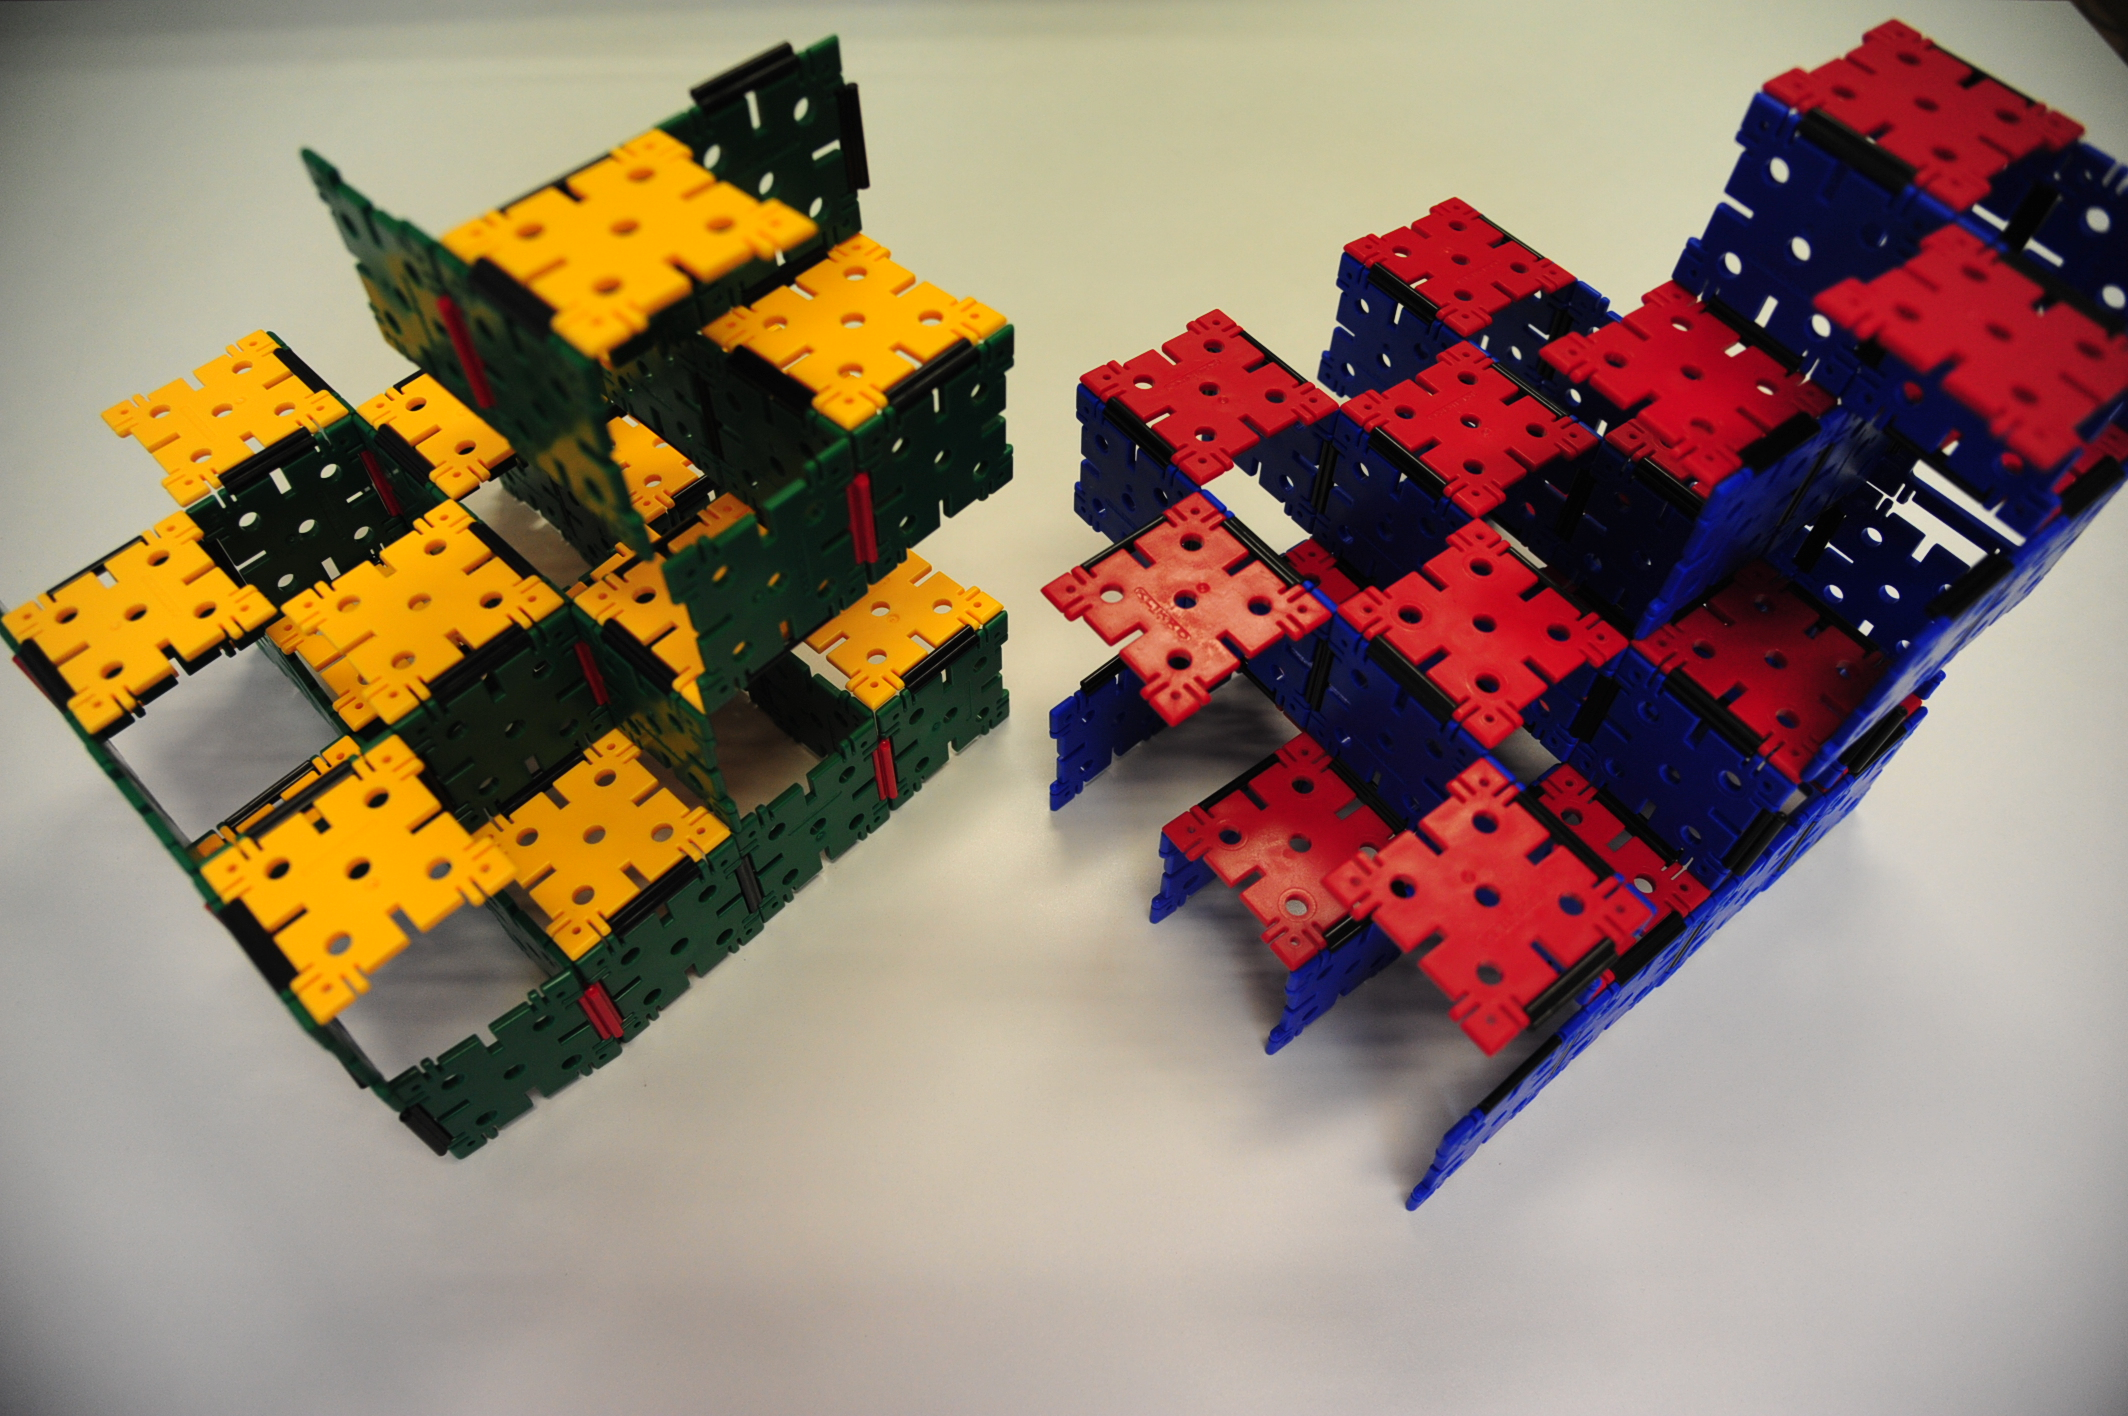
\includegraphics[height=4cm]{toys}
			%\end{center}
  \end{frame}
}


% Delete this, if you do not want the table of contents to pop up at
% the beginning of each subsection:

\begin{document}

\begin{frame}
  \titlepage
\end{frame}

\begin{frame}{Collaborators}
\begin{itemize}
%\item Yunqing Ouyang (欧阳云卿): Fudan University.
%\item Qing-Rui Wang (王晴睿): Chinese University of Hong Kong $\rightarrow$ Yale University.
%\item Zheng-Cheng Gu (顾正澄): Chinese University of Hong Kong.
\item Yunqing Ouyang: Fudan University $\rightarrow$ Huawei.
\item Qing-Rui Wang: YMSC, Tsinghua University.
\item Zheng-Cheng Gu: Chinese University of Hong Kong.
\begin{center}
	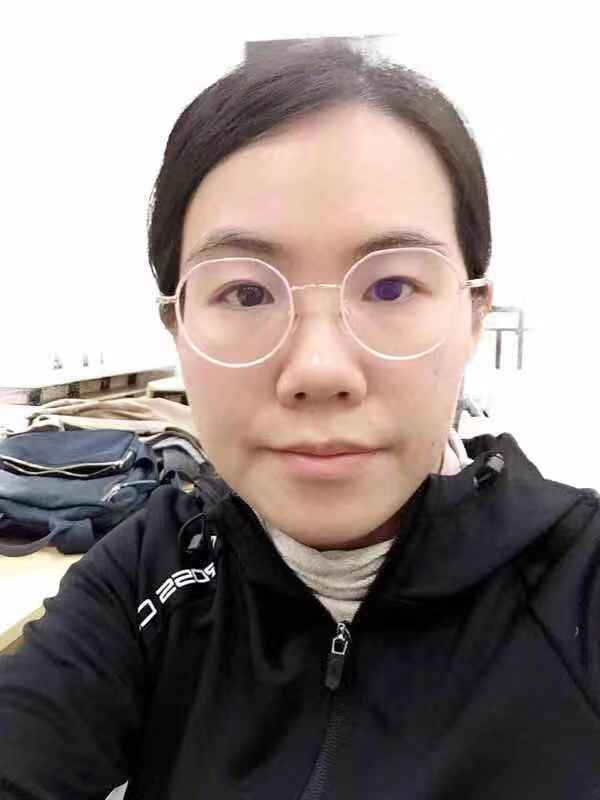
\includegraphics[height=3cm]{../people/yunqing}
	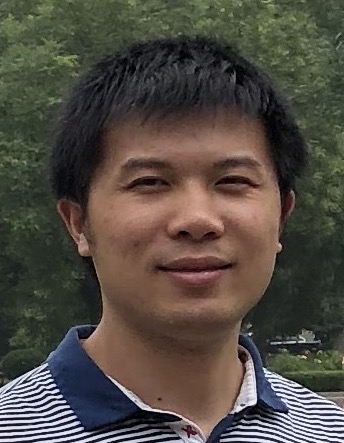
\includegraphics[height=3cm]{../people/qingrui}
	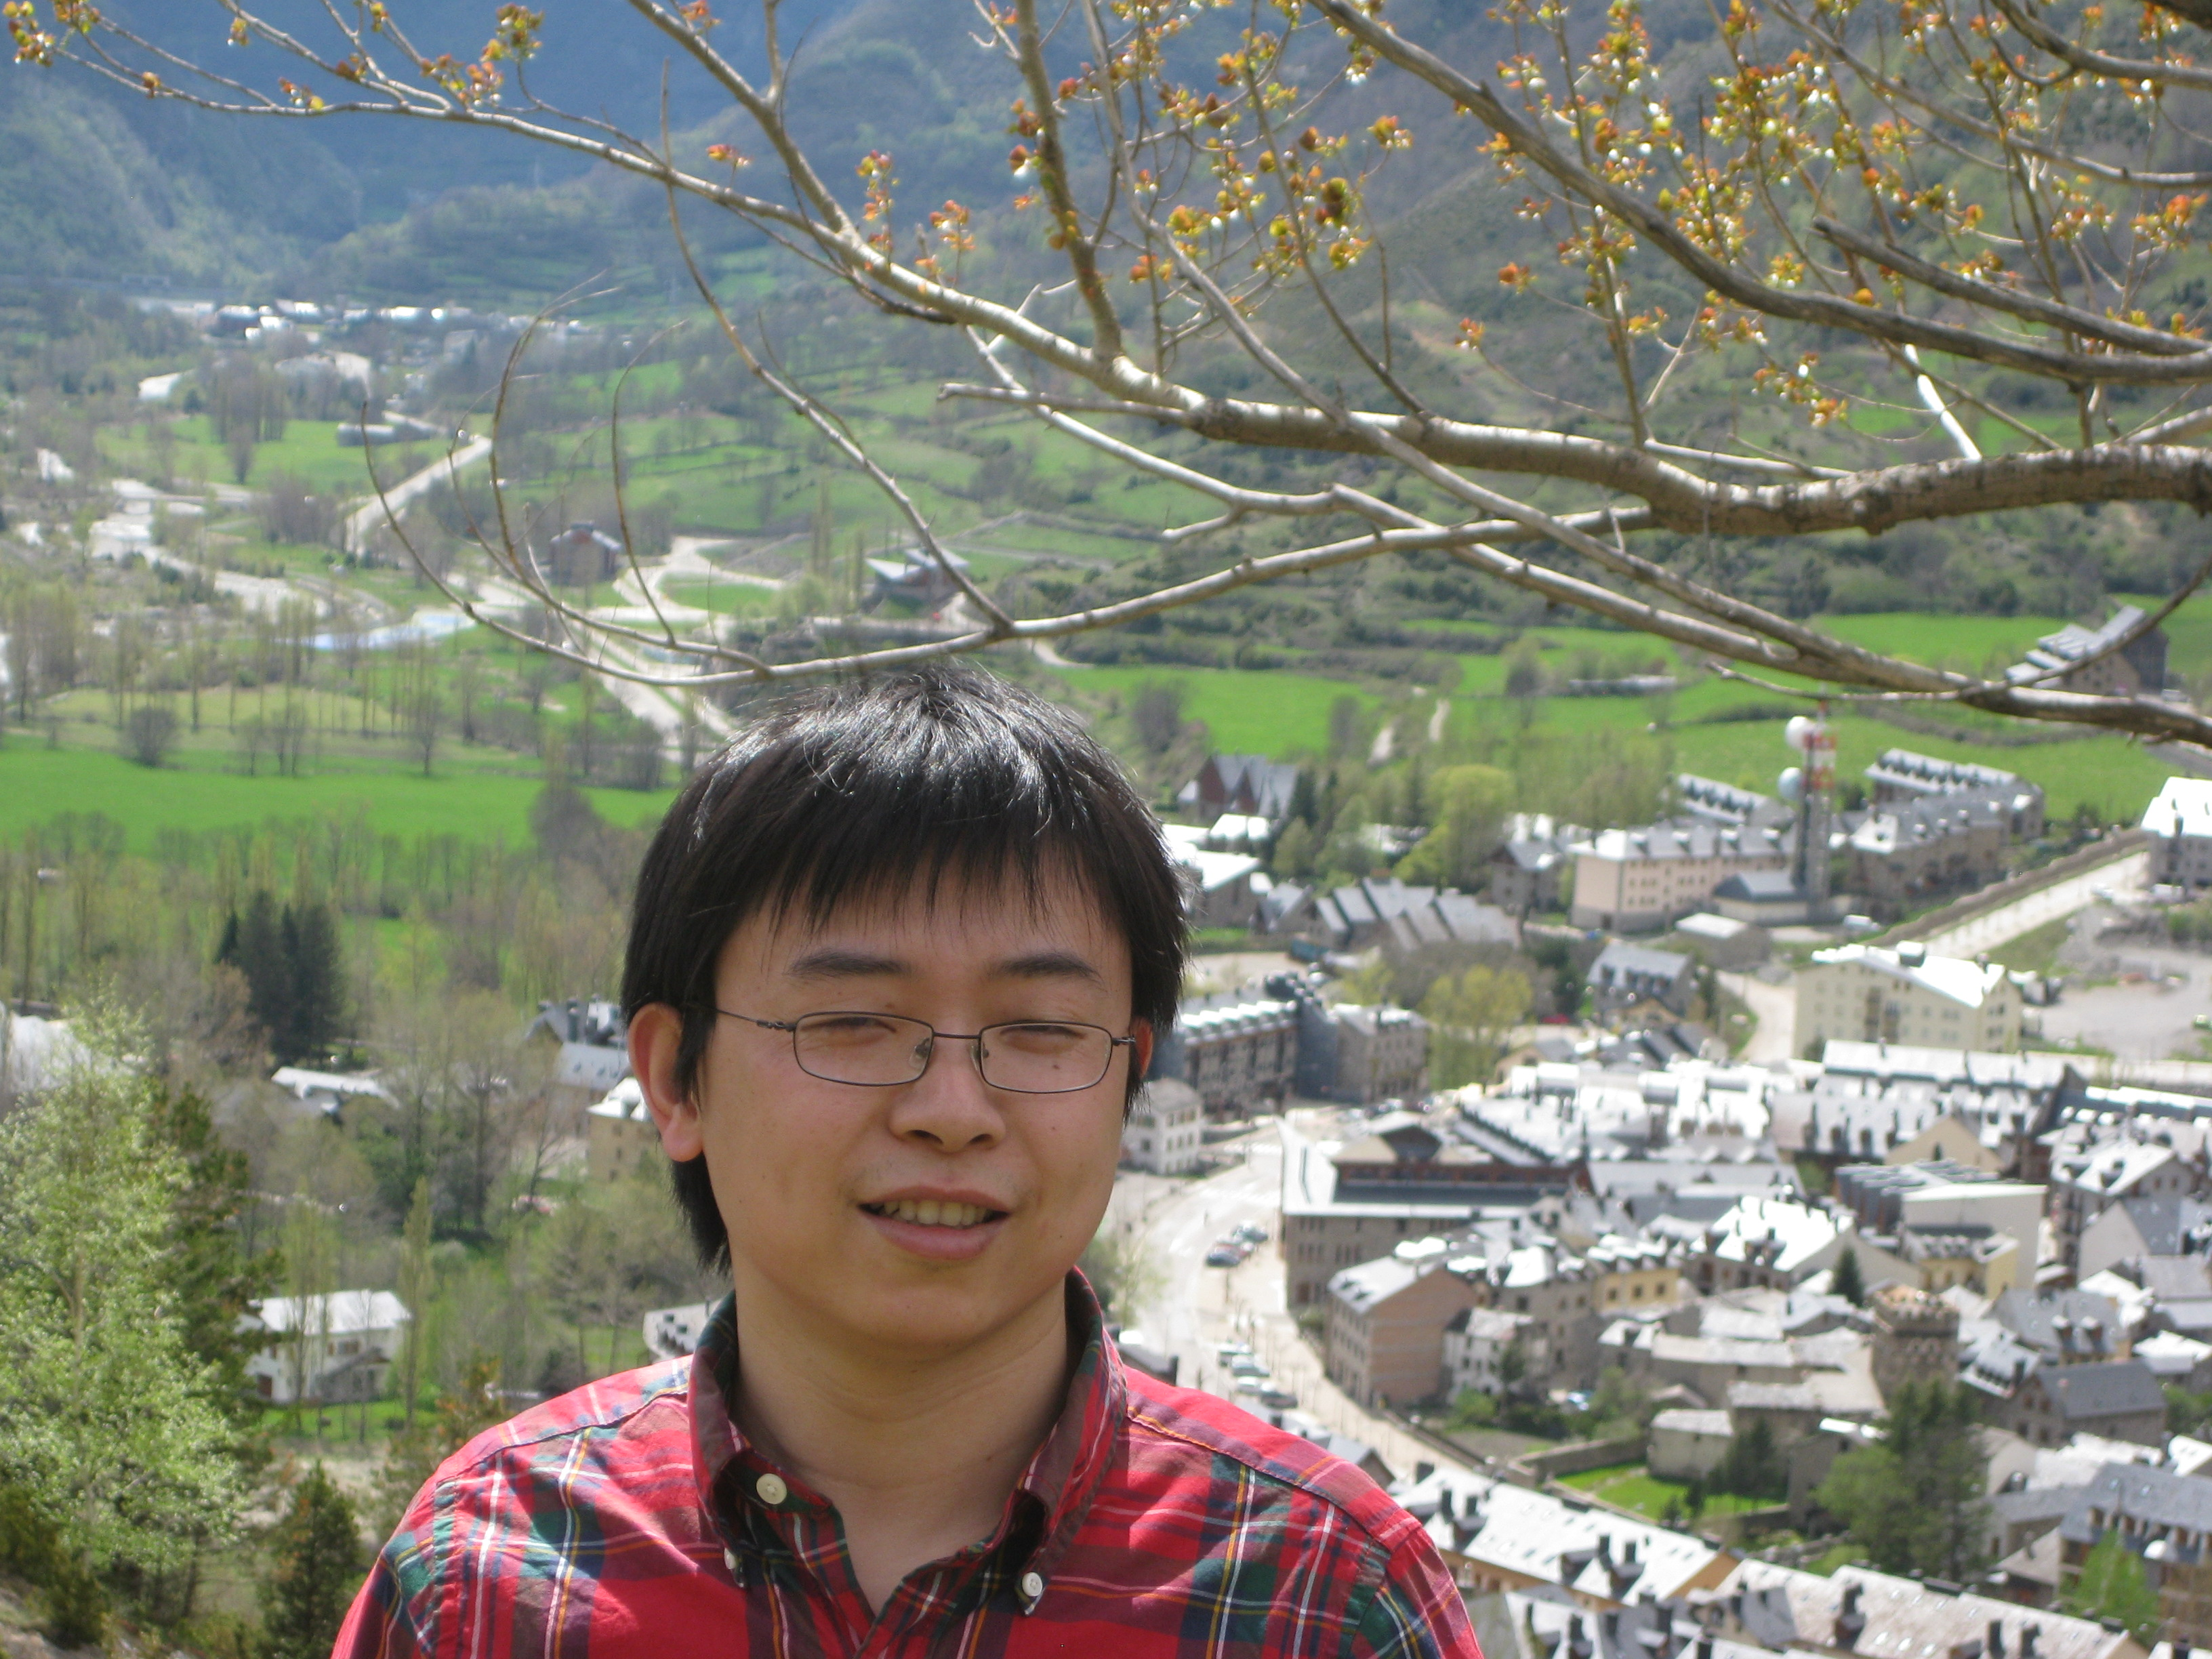
\includegraphics[height=3cm]{../people/zhengcheng}
\end{center}
\item Yunqing Ouyang, Qing-Rui Wang, Zheng-Cheng Gu and YQ,\\
Chin. Phys. Lett. \textbf{38}, 127101 (2021).
\item \url{https://github.com/yangqi137/SptSet}
\end{itemize}
\end{frame}

\section{Motivation: Why GAP?}

\begin{frame}
	\frametitle{The Problem: SPT and its classification}
	\begin{itemize}
		\item Symmetry-Protected Topological (SPT) States, examples: topological insulator (TI); Chern insulator, etc.
		\begin{center}
			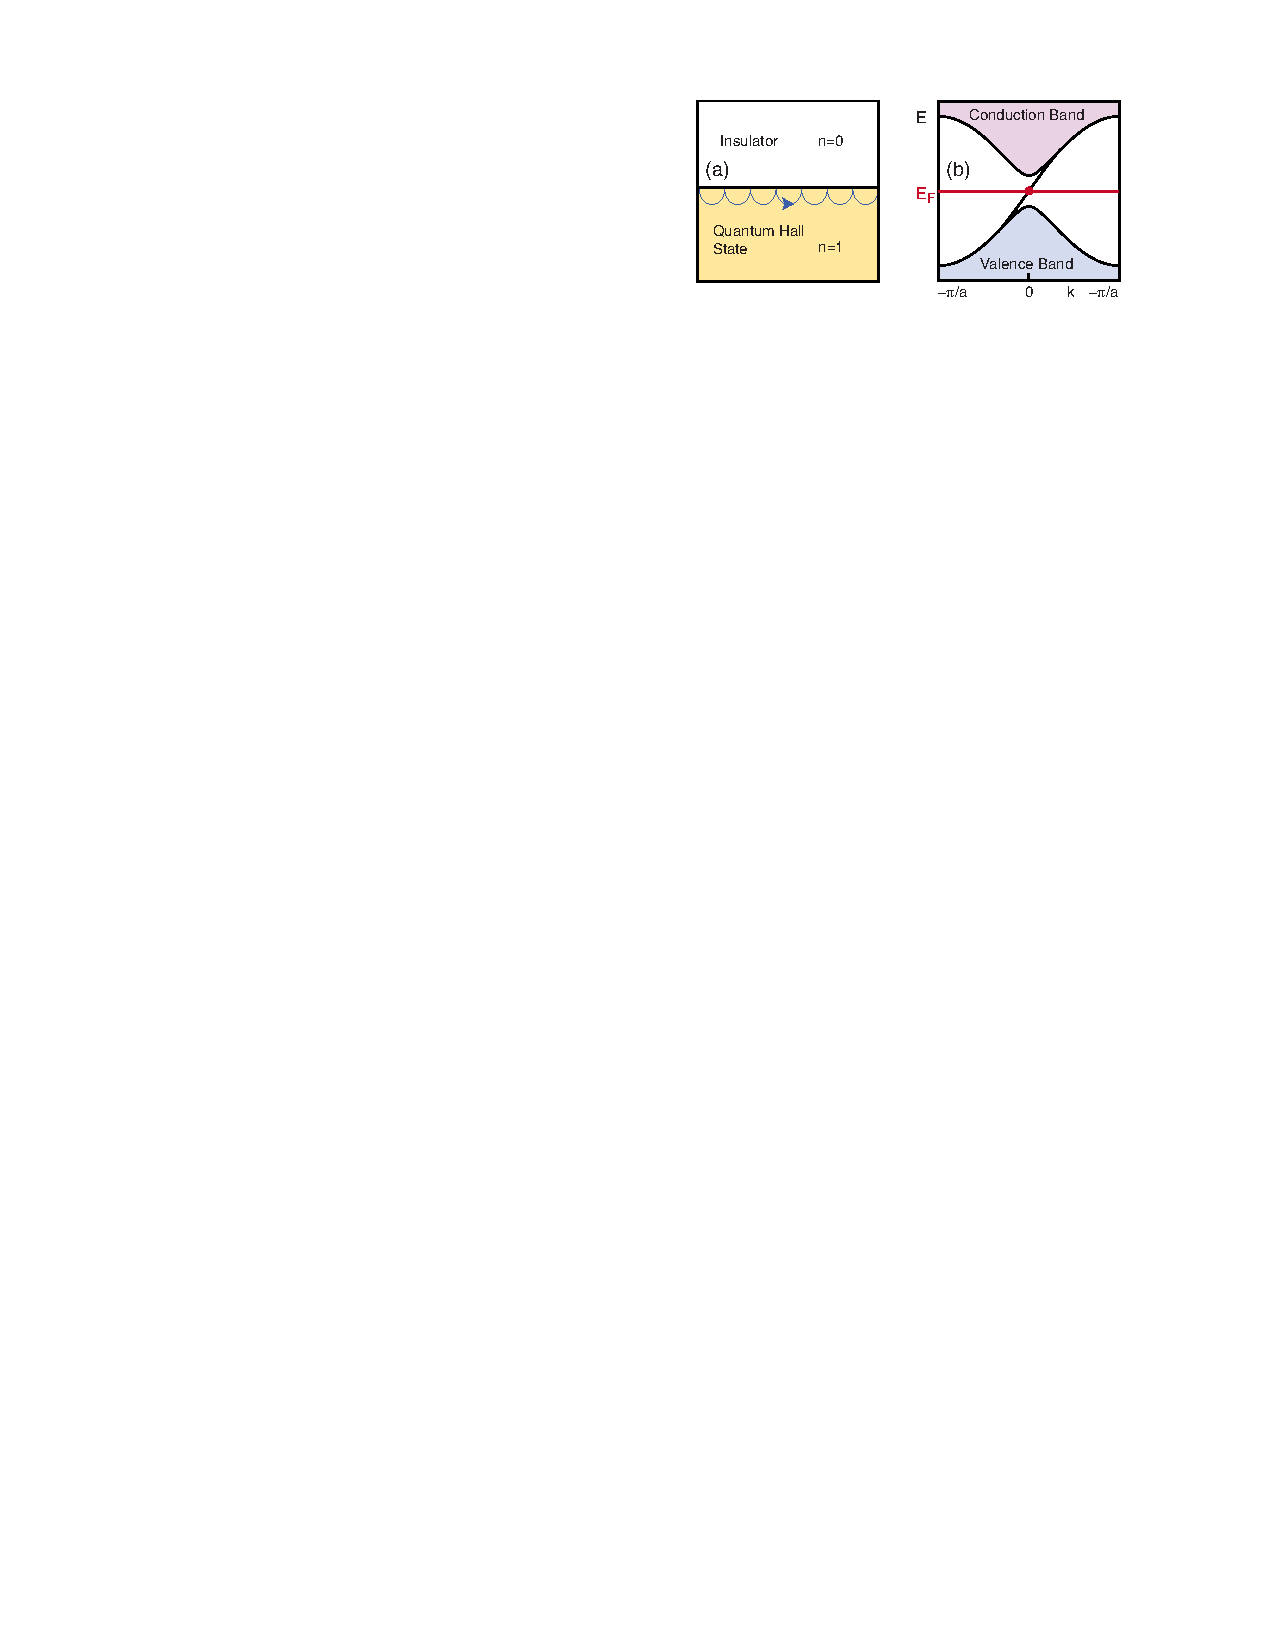
\includegraphics[width=6cm]{../spspt/qhe_edge}
		\end{center}
		{\small Classified by $\mathbb Z$: $[n]+[m]=[n+m]$; $[n]+[-n] = 0$.}	  
		\item SPT phases form an Abelian group under stacking.
		\item Classification is given by a generalized cohomology theory $\mathcal H^{d+1}(G)$,
		\begin{enumerate}
			\item Symmetry group $G$ (with more information...),
			\item Dimension $d$.
		\end{enumerate}
	\end{itemize}
\end{frame}

\begin{frame}[fragile]{Our solution: GAP}
	\begin{itemize}
		\item GAP = Group, Algorithm and Programming: \url{www.gap-system.org}.
		\item Advantage: easy to input of symmetry group.
		\begin{lstlisting}[basicstyle=\footnotesize]
			gap> G := CyclicGroup(4);
			pc group of size 4 with 2 generators>
			gap> G := DihedralGroup(6);
			pc group of size 4 with 2 generators>
			gap> G := SpaceGroup(3, 105);
			SpaceGroupOnRightBBNWZ( 3, 4, 5, 1, 2 )
		\end{lstlisting}
		\item Advantage: other algorithms related to group-cohomology calculation.			
	\end{itemize}
\end{frame}

\end{document}
